
\chapter{Wyniki działania algorytmu na popularnych zbiorach danych}

Lorem ipsum dolor sit amet, consectetur adipiscing elit. Nulla purus purus, fermentum in condimentum nec, sodales nec enim. Fusce auctor auctor porta. Proin tempus lacinia tortor, eget aliquam ante condimentum id. Morbi viverra congue posuere. Nunc non odio eros, sollicitudin pulvinar metus. Sed eget ligula ligula, a congue orci. Proin laoreet aliquet vulputate. Vivamus ut enim sed diam pretium fringilla. Class aptent taciti sociosqu ad litora torquent per conubia nostra, per inceptos himenaeos. Etiam convallis mi nec dolor pretium sed aliquam orci sagittis. Maecenas aliquam dictum neque vel mollis. Morbi vel vehicula mauris.

\section{Dokładność}
\begin{figure}[t]
    \begin{center}
        \begin{tabular}{ c c l }
            \toprule
            $j$ & $\textit{SA}[j]=i$ & $x[i..n-1]$ \\
            \midrule
            0 & 5 &        $\dollar$ \\
            1 & 4 &        o$\dollar$ \\
            2 & 1 &        orro$\dollar$ \\
            3 & 3 &        ro$\dollar$ \\
            4 & 2 &        rro$\dollar$ \\
            5 & 0 &        zorro$\dollar$ \\
            \bottomrule
        \end{tabular}
    \end{center}
\caption{Tablica sufiksów dla sufiksów ciągu ,,zorro\dollar''.}%
\label{rys:suffix-array-vis}
\end{figure}

\begin{figure}[t]
    \begin{center}
       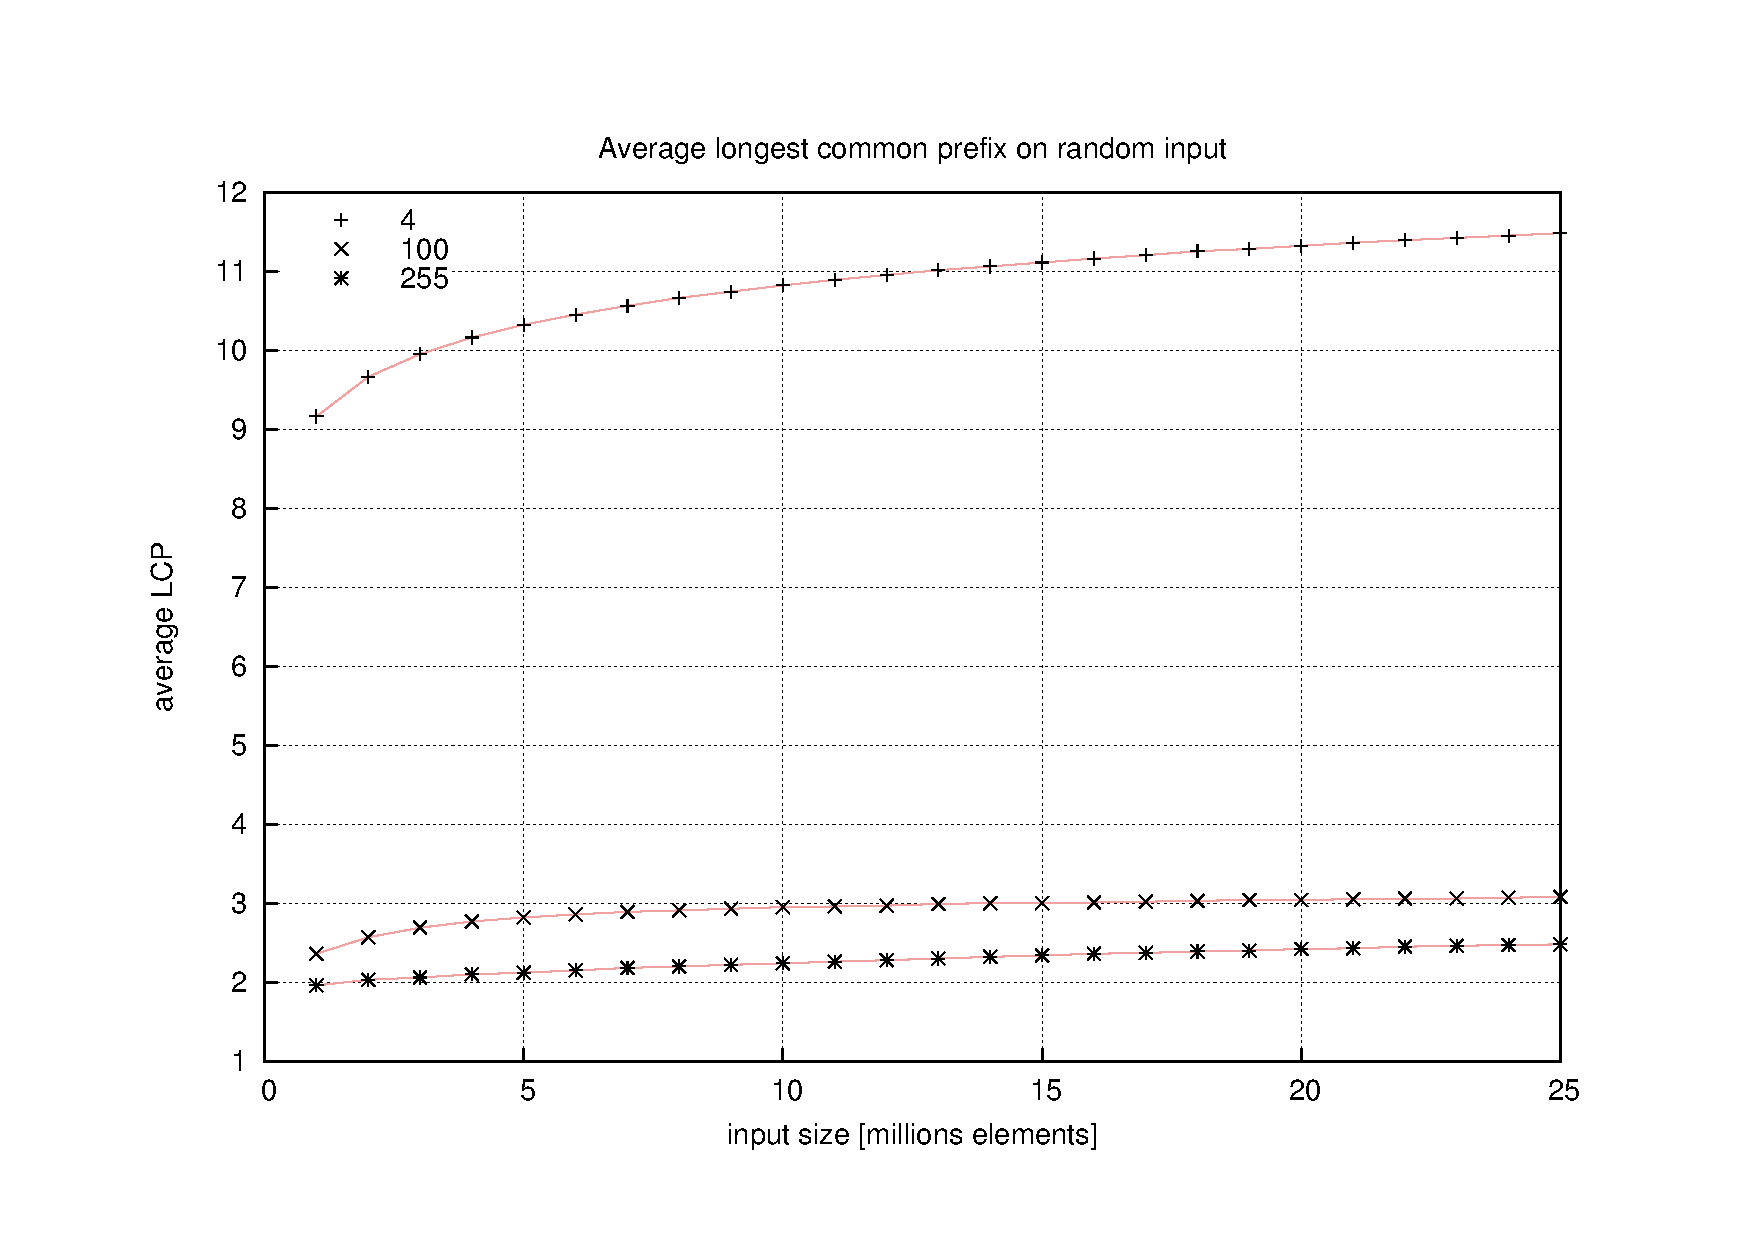
\includegraphics[scale=0.5]{figures/results/random-input-lcp.pdf}
    \end{center}

    \caption{Opis wykresu.}%
    \label{rys:wykres}
\end{figure}